% CS615 Aspects of System Administration
% Author: Jan Schaumann <jschauma@netmeister.org>
% $Id: slides.tex,v 1.6 2006/03/07 13:55:55 jschauma Exp $

\documentclass[xga]{xdvislides}
\usepackage[landscape]{geometry}
\usepackage{graphics}
\usepackage{graphicx}
\usepackage{colordvi}

\begin{document}
\setfontphv

%%% Headers and footers
\lhead{\slidetitle}                               % default:\lhead{\slidetitle}
\chead{CS615 - Aspects of System Administration}% default:\chead{\relax}
\rhead{Slide \thepage}                       % default:\rhead{\sectiontitle}
\lfoot{\Gray{SMTP, HTTP}}% default:\lfoot{\slideauthor}
\cfoot{\relax}                               % default:\cfoot{\relax}
\rfoot{\Gray{\today}}

\vspace*{\fill}
\begin{center}
	\Hugesize
		CS615 - Aspects of System Administration\\ [1em]
		SMTP, HTTP \\ [1em]
	\hspace*{5mm}\blueline\\ [1em]
	\Normalsize
		Department of Computer Science\\
		Stevens Institute of Technology\\
		Jan Schaumann\\
		\verb+jschauma@stevens-tech.edu+
		\verb+http://www.cs.stevens-tech.edu/~jschauma/615/+
\end{center}
\vspace*{\fill}

\subsection{Send me mail!}

\vspace*{\fill}
Start an EC2 instance and send a mail from it to {\tt
jschauma@stevens.edu} with a subject line of "CS615 - SMTP Exercise".
\vspace*{\fill}

\subsection{Email... still popular}
\begin{itemize}
	\item {\bf \~{}144 billion} – Average number of email messages per day.
	\item {\bf \~{}2.4 billion} – The number of email accounts worldwide.
	\item {\bf \~{}69\%} – The percentage of emails that were spam.
	\item {\bf \~{}0.22\%} – The percentage of emails that comprised some form of phishing attack.
\end{itemize}

\subsection{The Mail System}
Divided into
\begin{itemize}
	\item {\em Mail User Agent} or MUA, such as {\em mutt}, Mail.app, Outlook, ...
	\item {\em Mail Transfer Agent} or MTA, such as {\em postfix},
{\em sendmail}, {\em qmail}, ...
	\item {\em Mail Delivery Agent} or MDA, such as {\em procmail}
	\item {\em Access Agent} providing access via {\em POP}, {\em IMAP} etc.
\end{itemize}


\subsection{Sending email}
\begin{verbatim}
$ mail -s "Act I, Scene I" jschauma@stevens.edu
When shall we three meet again?
In thunder, lightning, or in rain?
^D
$
\end{verbatim}

\subsection{Anatomy of an email message}
\begin{verbatim}
Date: Sat, 29 Mar 2014 21:09:05 -0400 (EDT)
From: Jan Schaumann <jschauma@stevens.edu>
To: jschauma@stevens.edu
Subject: Act I, Scene I

When shall we three meet again?
In thunder, lightning, or in rain?

\end{verbatim}

\subsection{Anatomy of an email message}
An email consists of:
\begin{itemize}
	\item mandatory headers (such as "From ", "Delivered-To: ", ...)
	\item optional headers (such as "From: ", "To: ", "Subject: ", ...)
	\item the (optional) body of the message
\end{itemize}


\subsection{Anatomy of an email message}
\small
\begin{verbatim}
From jschauma@stevens.edu  Sat Mar 29 21:09:16 2014
Return-Path: jschauma@stevens.edu
X-Original-To: jschauma@netmeister.org
Delivered-To: jschauma@netmeister.org
Received: by panix.netmeister.org (Postfix, from userid 1004)
        id 0264A356ACC; Sat, 29 Mar 2014 21:09:15 -0400 (EDT)
Received: from na3sys009aog138.obsmtp.com (na3sys009aog138.obsmtp.com [74.125.149.19])
        by panix.netmeister.org (Postfix) with SMTP id 9F043356AAD
        for <jschauma@netmeister.org>; Sat, 29 Mar 2014 21:09:07 -0400 (EDT)
Received: from warp2.stevens.edu ([155.246.14.17]) by na3sys009aob138.postini.com ([74.125.148.12])
        with SMTP ID DSNKUzdus0U7/18n+gkoIEligpNCwWMOBR3u@postini.com; Sat, 29 Mar 2014 18:09:07 PDT
Received: from psmtp.com (na3sys009amx208.postini.com [74.125.149.48])
        by warp2.stevens.edu (Postfix) with SMTP id 36A7411FF51
        for <jschauma@stevens.edu>; Sat, 29 Mar 2014 21:09:06 -0400 (EDT)
Received: from na3sys009aog135.obsmtp.com ([74.125.149.84]) by na3sys009amx208.postini.com
        ([74.125.148.10]) with SMTP; Sat, 29 Mar 2014 18:09:06 PDT
Received: from nexus.stevens.edu ([155.246.14.12]) by na3sys009aob135.postini.com ([74.125.148.12])
        with SMTP ID DSNKUzdusST/Ao05xVu7tZO3NQJWYmKJRgAO@postini.com; Sat, 29 Mar 2014 18:09:06 PDT
Received: from avalon.srcit.stevens-tech.edu (gits.srcit.stevens-tech.edu [155.246.89.104])
        by nexus.stevens.edu (Postfix) with ESMTP id 8BA7A18237A
        for <jschauma@stevens.edu>; Sat, 29 Mar 2014 21:09:05 -0400 (EDT)
Received: by avalon.srcit.stevens-tech.edu (Postfix, from userid 10235)
        id 80768D6736; Sat, 29 Mar 2014 21:09:05 -0400 (EDT)
Subject: Act I, Scene I
To: jschauma@stevens.edu
X-Mailer: mail (GNU Mailutils 2.2)
Message-Id: <20140330010905.80768D6736@avalon.srcit.stevens-tech.edu>
Date: Sat, 29 Mar 2014 21:09:05 -0400 (EDT)
From: Jan Schaumann <jschauma@stevens.edu>

When shall we three meet again?
In thunder, lightning, or in rain?
\end{verbatim}
\Normalsize

\subsection{Sending email}
\begin{verbatim}
$ mail -s "Act I, Scene I" jschauma@stevens.edu
When shall we three meet again?
In thunder, lightning, or in rain?
^D
$
\end{verbatim}

\subsection{Who to hand the mail to?}
\newcommand{\smallish}{\fontsize{16}{16}\selectfont}
\begin{verbatim}
$ host -t mx stevens.edu
stevens.edu mail is handled by 20 stevens.edu.s9a2.psmtp.com.
stevens.edu mail is handled by 30 stevens.edu.s9b1.psmtp.com.
stevens.edu mail is handled by 10 stevens.edu.s9a1.psmtp.com.
stevens.edu mail is handled by 40 stevens.edu.s9b2.psmtp.com.
$
\end{verbatim}
\Normalsize

\subsection{By the way...}
\begin{verbatim}
$ whois psmtp.com
[...]
Registrant Name: DNS Admin
Registrant Organization: Google Inc.
Registrant Street: 1600 Amphitheatre Parkway
Registrant City: Mountain View
Registrant State/Province: CA
Registrant Postal Code: 94043
Registrant Country: US
Registrant Phone: +1.6502530000
Registrant Phone Ext:
Registrant Fax: +1.6506188571
[...]
\end{verbatim}

\subsection{Sending mail...}
\smallish
\begin{verbatim}
$ telnet stevens.edu.s9a1.psmtp.com 25
Trying 74.125.148.10...
Connected to stevens.edu.s9a1.psmtp.com.
Escape character is '^]'.
220 Postini ESMTP 202 y6_37_0c5 ready.  CA Business and Professions Code
Section 17538.45 forbids use of this system for unsolicited electronic
mail advertisements.
helo panix.netmeister.org
250 Postini says hello back
mail from: <jschauma@netmeister.org>
250 Ok
rcpt to: <jschauma@stevens.edu>
250 Ok
data
354 Feed me
Subject: Act I, Scene I

When shall we three meet again?
In thunder, lightning, or in rain?
.
250 Thanks
quit
221 Catch you later
Connection closed by foreign host.
\end{verbatim}
\Normalsize

\subsection{Sending the mail}
\begin{verbatim}
IP 166.84.7.99.51845 > 74.125.148.10.25: S 404385236:404385236(0)
IP 74.125.148.10.25 > 166.84.7.99.51845: S 1228051958:1228051958(0) ack 404385237
IP 166.84.7.99.51845 > 74.125.148.10.25: . ack 1
IP 74.125.148.10.25 > 166.84.7.99.51845: P 1:170(169) ack 1
IP 166.84.7.99.51845 > 74.125.148.10.25: P 1:28(27) ack 170
IP 74.125.148.10.25 > 166.84.7.99.51845: . ack 28
[...]
IP 74.125.148.10.25 > 166.84.7.99.51845: . ack 508
IP 74.125.148.10.25 > 166.84.7.99.51845: P 266:278(12) ack 508
IP 166.84.7.99.51845 > 74.125.148.10.25: P 508:514(6) ack 278
IP 166.84.7.99.51845 > 74.125.148.10.25: F 514:514(0) ack 278
IP 74.125.148.10.25 > 166.84.7.99.51845: . ack 514
IP 74.125.148.10.25 > 166.84.7.99.51845: P 278:299(21) ack 514
IP 74.125.148.10.25 > 166.84.7.99.51845: F 299:299(0) ack 514
IP 74.125.148.10.25 > 166.84.7.99.51845: . ack 515
\end{verbatim}
\Normalsize

\subsection{SMTP Codes}
SMTP codes consist of three digits in five classes:
\begin{itemize}
	\item {\bf 1xx} --  Mail server has accepted the command, but does not yet
		take any action. A confirmation message is required.
	\item {\bf 2xx} --  Mail server has completed the task successfully
		without errors.
	\item {\bf 3xx} --  Mail server has understood the request, but requires
		further information to complete it.
	\item {\bf 4xx} --  Mail server has encountered a temporary failure. If
		the command is repeated without any change, it might be
		completed. Try again, it may help!
	\item {\bf 5xx} --  Mail server has encountered a fatal error. Your
		request can't be processed.
\end{itemize}

\subsection{Receiving the mail}
\begin{verbatim}

IP 74.125.149.69.59141 > 166.84.7.99.25: S 1919605344:1919605344(0)
IP 166.84.7.99.25 > 74.125.149.69.59141: S 472727490:472727490(0) ack 1919605345
IP 74.125.149.69.59141 > 166.84.7.99.25: . ack 1
IP 166.84.7.99.52290 > 166.84.67.2.53: 10348+ PTR? 69.149.125.74.in-addr.arpa. (44)
IP 166.84.67.2.53 > 166.84.7.99.52290: 10348 1/4/4 (227)
IP 166.84.7.99.52289 > 166.84.67.2.53: 10349+ AAAA? na3sys009aog102.obsmtp.com. (44)
IP 166.84.67.2.53 > 166.84.7.99.52289: 10349 0/1/0 (110)
IP 166.84.7.99.52288 > 166.84.67.2.53: 10350+ A? na3sys009aog102.obsmtp.com. (44)
IP 166.84.67.2.53 > 166.84.7.99.52288: 10350 1/4/4 (203)
IP 166.84.7.99.25 > 74.125.149.69.59141: P 1:41(40) ack 1
IP 74.125.149.69.59141 > 166.84.7.99.25: . ack 41
[...]
IP 74.125.149.69.59141 > 166.84.7.99.25: P 71:106(35) ack 81
IP 166.84.7.99.52287 > 166.84.67.2.53: 10351+ A? na3sys009aog102.obsmtp.com. (44)
IP 166.84.67.2.53 > 166.84.7.99.52287: 10351 1/4/4 (203)
IP 166.84.7.99.52286 > 166.84.67.2.53: 10352+ A? 69.149.125.74.sbl.spamhaus.org. (48)
IP 166.84.67.2.53 > 166.84.7.99.52286: 10352 NXDomain 0/1/0 (104)
IP 166.84.7.99.52285 > 166.84.67.2.53: 10353+ A? 69.149.125.74.bl.spamcop.net. (46)
IP 166.84.67.2.53 > 166.84.7.99.52285: 10353 NXDomain 0/1/0 (99)
IP 166.84.7.99.25 > 74.125.149.69.59141: P 81:95(14) ack 106
IP 74.125.149.69.59141 > 166.84.7.99.25: . ack 95
IP 74.125.149.69.59141 > 166.84.7.99.25: P 106:112(6) ack 95
IP 166.84.7.99.25 > 74.125.149.69.59141: P 95:132(37) ack 112
IP 74.125.149.69.59141 > 166.84.7.99.25: . ack 132
IP 74.125.149.69.59141 > 166.84.7.99.25: P 112:1276(1164) ack 132
IP 166.84.7.99.25 > 74.125.149.69.59141: . ack 1276
IP 74.125.149.69.59141 > 166.84.7.99.25: P 1276:1348(72) ack 132
IP 166.84.7.99.25 > 74.125.149.69.59141: P 132:169(37) ack 1348
IP 166.84.7.99.25 > 74.125.149.69.59141: P 169:184(15) ack 1354
IP 166.84.7.99.25 > 74.125.149.69.59141: F 184:184(0) ack 1354
IP 74.125.149.69.59141 > 166.84.7.99.25: F 1354:1354(0) ack 184
IP 166.84.7.99.25 > 74.125.149.69.59141: . ack 1355
IP 74.125.149.69.59141 > 166.84.7.99.25: . ack 185
\end{verbatim}
\Normalsize

\subsection{Service Considerations}

\begin{itemize}
	\item outsourcing versus in-house
	\item privacy considerations
	\item spam protections
	\item phishing protections
	\item mail delivery cannons for notifications vs. spam lists
	\item high volume traffic demands fine-tuned systems
	\item high volume traffic implications on logging
\end{itemize}

{\tt http://is.gd/JQp1zM}

\newpage
\vspace*{\fill}
\begin{center}
	\Hugesize
		Hypertext Transfer Protocol\\ [1em]
	\hspace*{5mm}
	\blueline\\
	\hspace*{5mm}\\
		Today's Universal Internet Pipe
\end{center}
\vspace*{\fill}

\subsection{Set up an HTTP server.}

\vspace*{\fill}
Start an EC2 instance and set up an HTTP server to listen on port 8080.
Add a simple index.html file containing your username.

When done, paste the full URL (ie http:///) into the class IRC channel
\#cs615asa.

{\tt https://webchat.freenode.net/}
\vspace*{\fill}


\subsection{HTTP: Hypertext}
\vspace{.5in}
\begin{center}
	\Huge
	W W W
	\\
\vspace{.5in}
	{\em ``The World Wide Web is the only thing I know of whose shortened form
	takes three times longer to say than what it's short for.'' -- Douglas Adams}
\end{center}
\Normalsize


\subsection{HTTP: Hypertext}
\begin{center}
	\includegraphics[scale=0.9]{pics/http-proposal-detail.eps} \\
	\vspace{.5in}
	\verb+http://is.gd/JnZaN6+
\end{center}

\subsection{HTTP}
\vspace{.5in}
\begin{center}
	\Huge
	Hypertext Transfer Protocol
	\\
	\vspace{.5in}
	RFC2616
\end{center}
\Normalsize

\subsection{HTTP}
\vspace{.5in}
\begin{center}
	\Huge
	HTTP is a request/response protocol.
\end{center}
\Normalsize

\subsection{The Hypertext Transfer Protocol}
HTTP is a request/response protocol:
\begin{enumerate}
	\item client sends a request to the server
	\item server responds
\end{enumerate}

\subsection{The Hypertext Transfer Protocol}
HTTP is a request/response protocol:
\begin{enumerate}
	\item client sends a request to the server
		\begin{itemize}
			\item request method
			\item URI
			\item protocol version
			\item request modifiers
			\item client information
		\end{itemize}
	\item server responds
\end{enumerate}

\subsection{HTTP: A client request}
\vspace*{.5in}
\\
\Hugesize
\begin{center}
\begin{verbatim}
$ telnet www.google.com 80
Trying 173.194.75.147...
Connected to www.google.com.
Escape character is '^]'.
GET / HTTP/1.0
\end{verbatim}
\end{center}
\Normalsize
\vspace*{\fill}


\subsection{The Hypertext Transfer Protocol}
HTTP is a request/response protocol:
\begin{enumerate}
	\item client sends a request to the server
		\begin{itemize}
			\item request method
			\item URI
			\item protocol version
			\item request modifiers
			\item client information
		\end{itemize}
	\item server responds
		\begin{itemize}
			\item status line (including success or error code)
			\item server information
			\item entity metainformation
			\item content
		\end{itemize}
\end{enumerate}

\subsection{HTTP: a server response}
%\smallish
\begin{verbatim}
HTTP/1.0 200 OK
Date: Sun, 31 Mar 2013 01:54:40 GMT
Set-Cookie: PREF=ID=c5eb56d629b347cc:FF=0:TM=1364694880:LM=1364694880:
S=sIdRFdxV9YvtQOlG; expires=Tue, 31-Mar-2015 01:54:40 GMT; path=/;
domain=.google.com
Set-Cookie: NID=67=hvBnOob2NoZW4haTJVfajbcyn_jips50lKRe-8nawzdCZ6AukNR
_s8CNHD6ZA-Z2721nA3TpLrNXt-2zyIui23j4kdsdF8Gg--PmGsMOJ3Jv5frEzQG1elHJv92HL-w2;
expires=Mon, 30-Sep-2013 01:54:40 GMT; path=/; domain=.google.com; HttpOnly
Server: gws

<!doctype html><html itemscope="itemscope" itemtype="http://schema.org/WebPage">
<head><meta content="Search the...

\end{verbatim}
%\Normalsize

\subsection{The Hypertext Transfer Protocol}
Server status codes:
\begin{itemize}
	\item {\bf 1xx} -- Informational; Request received, continuing process
	\item {\bf 2xx} -- Success; The action was successfully received,
        understood, and accepted
	\item {\bf 3xx} -- Redirection; Further action must be taken in order to
        complete the request
	\item {\bf 4xx} -- Client Error; The request contains bad syntax or
		cannot be fulfilled
	\item {\bf 5xx} -- Server Error; The server failed to fulfill an
		apparently valid request
\end{itemize}

\subsection{HTTP: A client request}
\smallish
\begin{verbatim}
$ telnet www.cs.stevens.edu 80
Trying 155.246.89.84...
Escape character is '^]'.
GET / HTTP/1.0

HTTP/1.1 302 Found
Date: Mon, 01 Apr 2013 20:58:35 GMT
Server: Apache/2.2.16 (Debian)
Location: http://www.stevens.edu/compsci
Vary: Accept-Encoding
Content-Length: 312
Content-Type: text/html; charset=iso-8859-1

<!DOCTYPE HTML PUBLIC "-//IETF//DTD HTML 2.0//EN">
<html><head>
<title>302 Found</title>
</head><body>
<h1>Found</h1>
<p>The document has moved <a
href="http://www.stevens.edu/compsci">here</a>.</p>
<hr>
<address>Apache/2.2.22 (Debian) Server at www.cs.stevens.edu Port
80</address>
</body></html>
\end{verbatim}
\Normalsize

\subsection{HTTP: A client request}
\smallish
\begin{verbatim}
$ telnet www.stevens.edu 80
Trying 54.243.80.146...
Connected to mc-4471-1746286150.us-east-1.elb.amazonaws.com.
Escape character is '^]'.
GET /compsci HTTP/1.0

HTTP/1.1 404 Not Found
Accept-Ranges: bytes
Age: 0
Content-Type: text/html
Date: Sun, 30 Mar 2014 01:46:50 GMT
Server: nginx
Via: 1.1 varnish
X-Cache: MISS
X-Varnish: 2034677690
Content-Length: 971
Connection: Close
\end{verbatim}
\Normalsize

\subsection{HTTP: A client request}
\smallish
\begin{verbatim}
$ telnet www.stevens.edu 80
Trying 54.243.80.146...
Connected to mc-4471-1746286150.us-east-1.elb.amazonaws.com.
Escape character is '^]'.
GET /compsci HTTP/1.1
Host: www.stevens.edu

HTTP/1.1 301 Moved Permanently
Content-Type: text/html; charset=iso-8859-1
Date: Sun, 30 Mar 2014 01:49:12 GMT
Expires: Thu, 10 Apr 2014 01:29:25 GMT
Location: http://web.stevens.edu/compsci
Server: nginx
Content-Length: 238
Connection: keep-alive

<!DOCTYPE HTML PUBLIC "-//IETF//DTD HTML 2.0//EN">
<html><head>
<title>301 Moved Permanently</title>
</head><body>
<h1>Moved Permanently</h1>
<p>The document has moved <a
href="http://web.stevens.edu/compsci">here</a>.</p>
</body></html>
\end{verbatim}
\Normalsize

\subsection{HTTP: A client request}
\smallish
\begin{verbatim}
$ telnet web.stevens.edu 80
Trying 155.246.21.84...
Connected to rweb.cc.stevens.edu.
Escape character is '^]'.
GET /compsci HTTP/1.1
Host: web.stevens.edu

HTTP/1.1 301 Moved Permanently
Date: Sun, 30 Mar 2014 01:50:36 GMT
Server: Apache/2.2.16 (Debian)
Location: http://web.stevens.edu/compsci/
Content-Length: 320
Content-Type: text/html; charset=iso-8859-1

<!DOCTYPE HTML PUBLIC "-//IETF//DTD HTML 2.0//EN">
<html><head>
<title>301 Moved Permanently</title>
</head><body>
<h1>Moved Permanently</h1>
<p>The document has moved <a
href="http://web.stevens.edu/compsci/">here</a>.</p>
<hr>
<address>Apache/2.2.16 (Debian) Server at web.stevens.edu Port
80</address>
\end{verbatim}
\Normalsize

\subsection{HTTP: A client request}
\smallish
\begin{verbatim}
$ telnet web.stevens.edu 80
Trying 155.246.21.84...
Connected to rweb.cc.stevens.edu.
Escape character is '^]'.
GET /compsci/ HTTP/1.1
Host: web.stevens.edu

HTTP/1.1 302 Moved Temporarily
Date: Sun, 30 Mar 2014 01:52:03 GMT
Server: Apache/2.2.16 (Debian)
X-Powered-By: PHP/5.3.3-7+squeeze8
location: home.php
Vary: Accept-Encoding
Content-Length: 0
Content-Type: text/html
Via: 1.1 www.stevens.edu
\end{verbatim}

\subsection{HTTP: A client request}
\smallish
\begin{verbatim}
$ telnet web.stevens.edu 80
Trying 155.246.21.84...
Connected to rweb.cc.stevens.edu.
Escape character is '^]'.
GET /compsci/home.php HTTP/1.1
Host: web.stevens.edu

HTTP/1.1 200 OK
Date: Sun, 30 Mar 2014 01:53:23 GMT
Server: Apache/2.2.16 (Debian)
X-Powered-By: PHP/5.3.3-7+squeeze8
Vary: Accept-Encoding
Content-Type: text/html
Via: 1.1 www.stevens.edu
Transfer-Encoding: chunked

1e3a
<!DOCTYPE html
	PUBLIC "-//W3C//DTD HTML 4.0 Transitional//EN">
<html>
<head>

\end{verbatim}

\subsection{Slightly easier...}
\begin{center}
	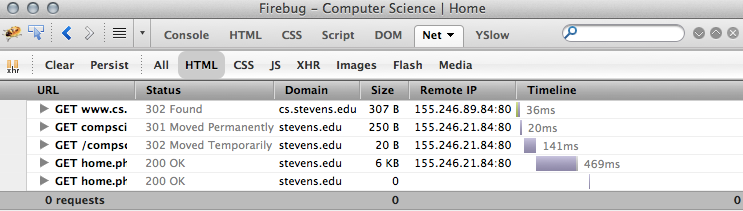
\includegraphics[scale=0.7]{pics/firebug.eps}
\end{center}
\addvspace{.25in}
\begin{center}
	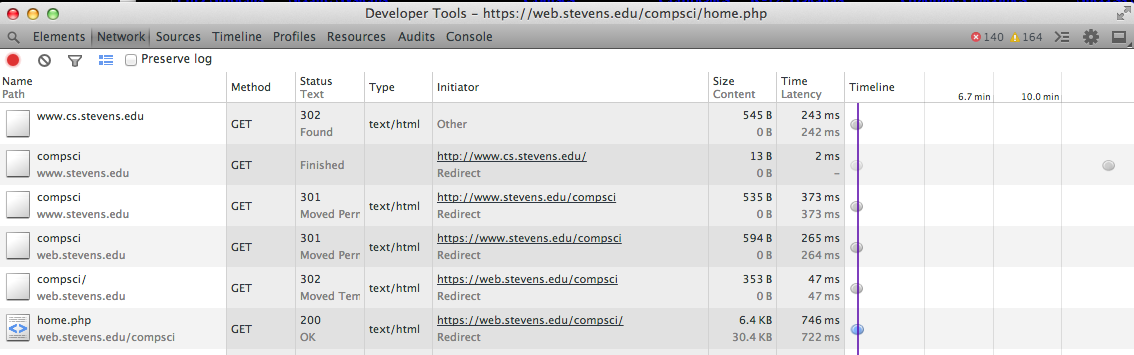
\includegraphics[scale=0.5]{pics/chrome-tools.eps}
\end{center}




\subsection{HTTP - more than just text}
HTTP is a {\em Transfer Protocol} -- serving {\em data}, not any specific
text format.

\begin{itemize}
	\item {\tt Accept-Encoding} client header can specify different formats
		such as {\em gzip}, {\em Shared Dictionary Compression over HTTP (SDCH)} etc.
	\item corresponding server headers: {\tt Content-Type} and
		{\tt Content-Encoding}
\end{itemize}
\begin{center}
	
\includegraphics[scale=2.0]{pics/datatransfer.eps}
\end{center}

\subsection{HTTP - more than just static data}
HTTP is a {\em Transfer Protocol} -- what is transferred need not be
static; resources may generate different data to return based on many
variables.

\begin{itemize}
	\item CGI -- resource is {\em executed}, needs to generate
		appropriate response headers
	\item server-side scripting (ASP, PHP, Perl, ...)
	\item client-side scripting (JavaScript/ECMAScript/JScript,...)
	\item applications based on HTTP, using:
		\begin{itemize}
			\item AJAX
			\item RESTful services
			\item JSON, XML, YAML to represent state and
				abstract information
		\end{itemize}
\end{itemize}

%\subsection{HTTPS}
%HTTPS == HTTP over SSL or TLS
%\begin{itemize}
%	\item use of a different server port (443)
%	\item basically use of HTTP protocol just as with plain TCP
%	\item connection initiation:
%		\begin{itemize}
%			\item client initiates a connection to the server
%			\item client sends TLS ClientHello
%			\item client and server perform TLS handshake (according to TLS
%				protocol (RFC 2246))
%			\item client makes regular HTTP requests
%		\end{itemize}
%\end{itemize}
%
%\subsection{Crypto is hard, let's go shopping!}
%Use of SSL has a performance impact:
%\begin{itemize}
%	\item each handshake requires compute-intensive (asymmetric
%		cryptography) certificate
%	\item each session then uses the less intense (symmetric
%		cryptogaphy) session key
%	\item processor-intensive public key encryption algorithms can be
%		offloaded to so-called {\em Crypto Accelerator} cards
%\end{itemize}
%\begin{center}
%	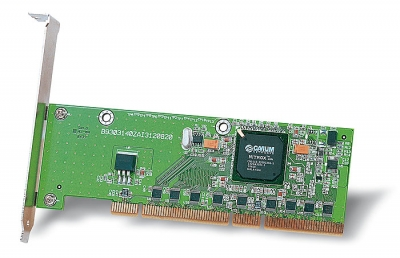
\includegraphics[scale=0.7]{pics/crypto-accelerator.eps}
%\end{center}
%
\subsection{HTTP overload}
Ways to mitigate HTTP overload:

\begin{itemize}
	\item DNS round-robin to many web servers
	\item load balancing
	\item web cache / accelerators
	\item content delivery networks
\end{itemize}

These solutions depend on the location within the network and the scale of
the environment.

\subsection{Load Balancing}
\begin{center}
	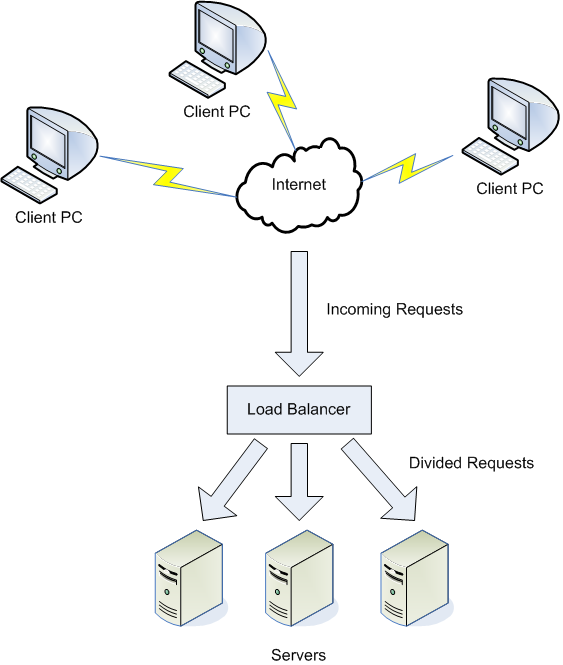
\includegraphics[scale=0.55]{pics/Lb101.eps}
\end{center}

\subsection{Load Balancing: Inbound}
\begin{center}
	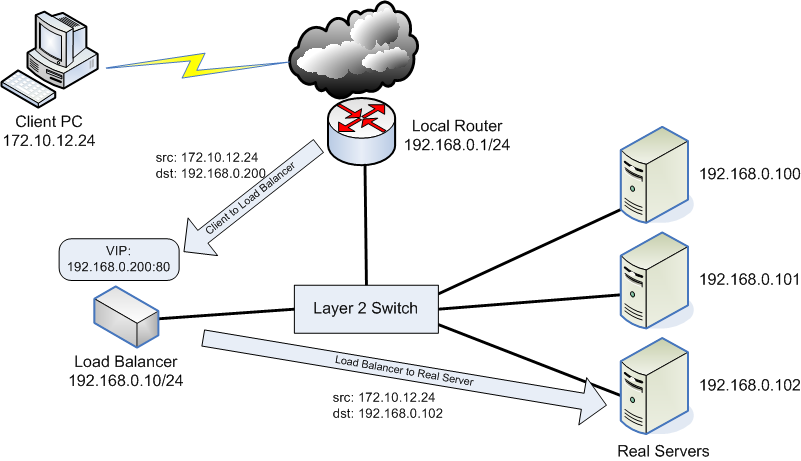
\includegraphics[scale=0.7]{pics/One-armed-inbound.eps}
\end{center}

\subsection{Load Balancing: Outbound}
\begin{center}
	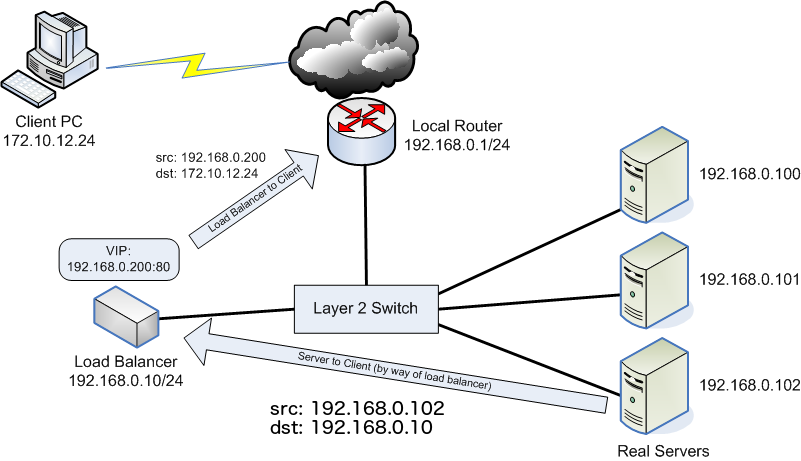
\includegraphics[scale=0.7]{pics/One-armed-outbound.eps}
\end{center}

\subsection{Load Balancing: Direct Server Return}
\begin{center}
	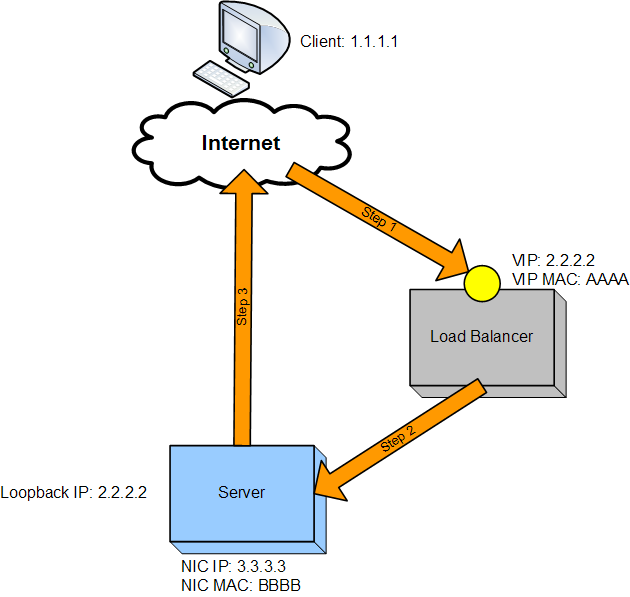
\includegraphics[scale=0.6]{pics/DSR.eps}
\end{center}

\subsection{Content Delivery Networks}
\begin{center}
	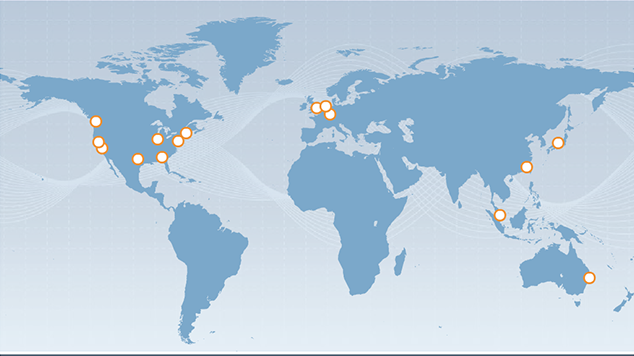
\includegraphics[scale=0.9]{pics/cdn.eps}
\end{center}

\subsection{Content Delivery Networks}
\begin{itemize}
	\item cache content in strategic locations
	\item determine location to serve from via geomapping of IP
		addresses (beware IPv6 aggregation!)
	\item often uses a separate domain to distinguish small
		objects/large objects or dynamic content/static content
	\item either out-sourced or in-house (if your organization is a
		Tier-1 or Tier-2 peering partner)
	\item request routing happens via Global Server Load Balancing,
		DNS-based request routing, anycasting etc.
	\item provides vast amounts of interesting data about your clients
		(see \verb+http://www.akamai.com/stateoftheinternet/+)
\end{itemize}

%\subsection{In-class exercise}
%\vspace{1in}
%\verb+http://www.cs.stevens.edu/~jschauma/615/http-exercise.html+


\subsection{Reading}
SMTP:
\begin{itemize}
	\item \verb+http://bit.ly/5zIadJ+
	\item RFC 821, 2821
	\item \verb+aliases(5)+, \verb+mail(1)+
	\item \verb+sendmail(8)+, \verb+postfix(8)+
\end{itemize}

\subsection{Reading}
HTTP etc.:
\begin{itemize}
	\item RFC 2616, 2818, 3875
	\item \verb+http://httpd.apache.org/docs/+
	\item \verb+http://www.w3.org/Protocols/+
	\item REST: \verb+http://is.gd/leSvGa+
	\item CDNs: \verb+http://is.gd/R5DoxA+
		\begin{itemize}
			\item \verb+http://www.edgecast.com/+
			\item \verb+https://aws.amazon.com/cloudfront/+
			\item \verb+http://www.akamai.com/+
			\item \verb+http://www.limelight.com/+
			\item ...
		\end{itemize}
	\item \verb+http://developer.yahoo.com/performance/rules.html+
\end{itemize}



\end{document}
